\section{RRTGoal\-Zoom  Class Reference}
\label{class_RRTGoalZoom}\index{RRTGoalZoom@{RRTGoal\-Zoom}}
Bias the samples toward the goal as the tree gets closer. 


{\tt \#include $<$rrt.h$>$}

Inheritance diagram for RRTGoal\-Zoom::\begin{figure}[H]
\begin{center}
\leavevmode
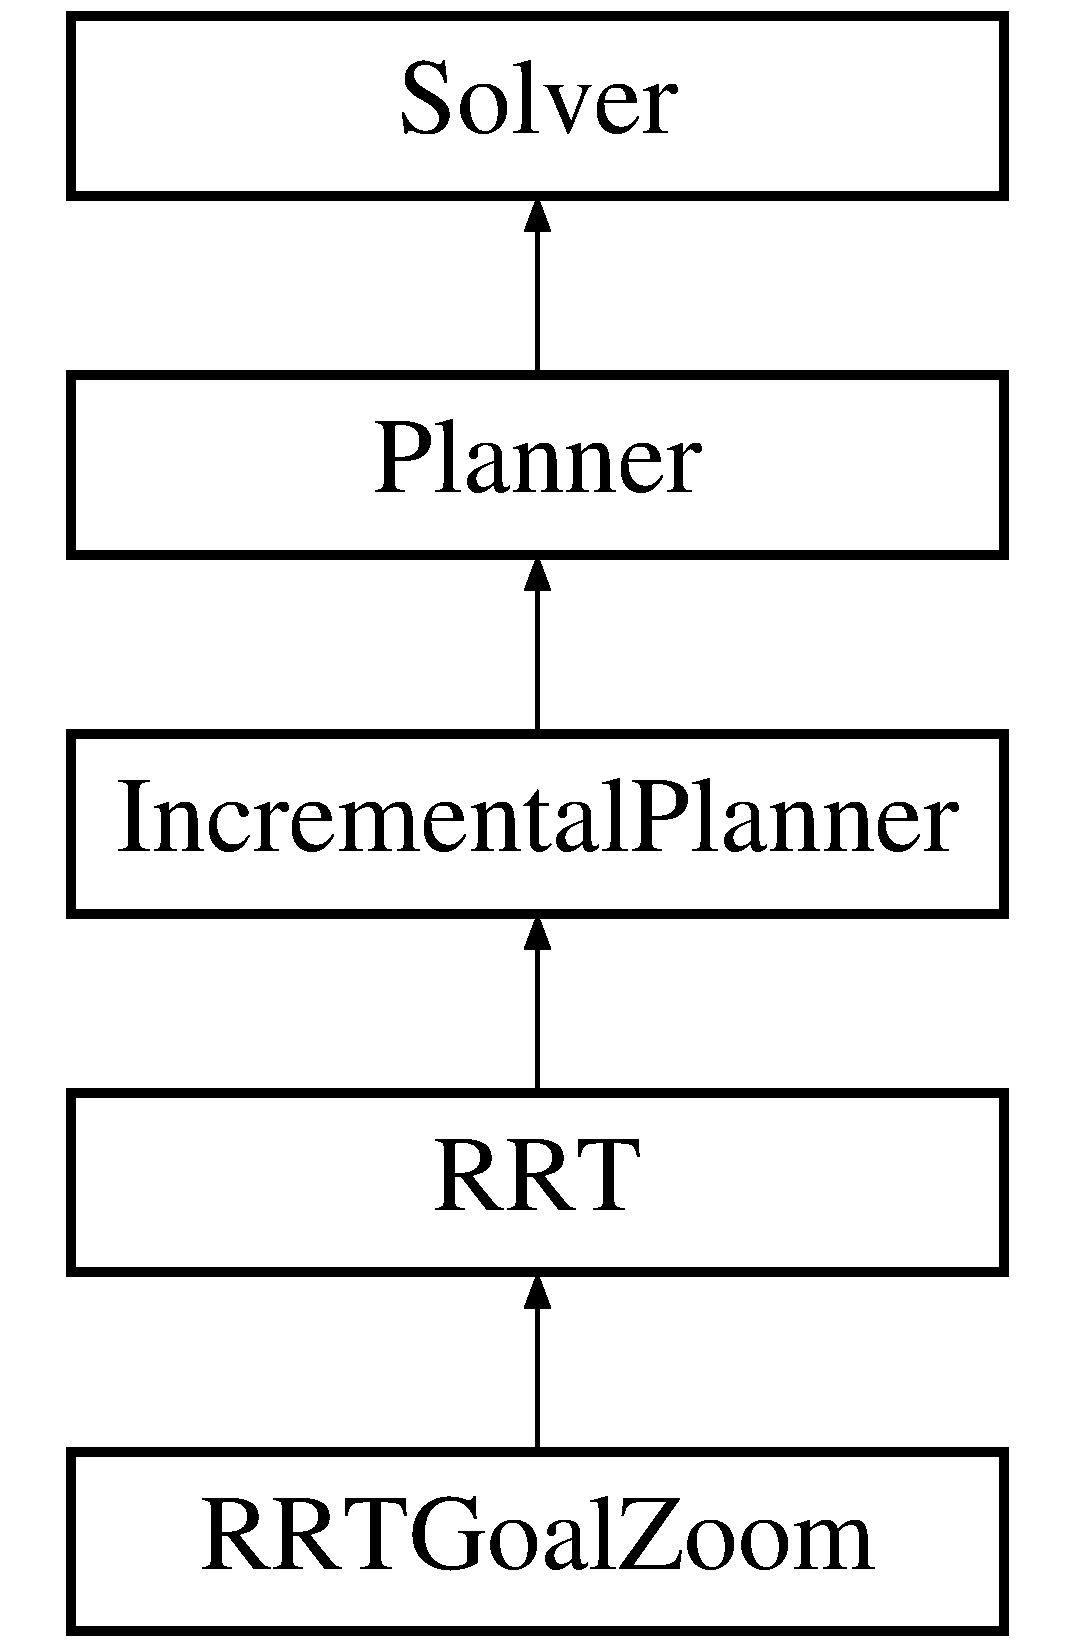
\includegraphics[height=5cm]{class_RRTGoalZoom}
\end{center}
\end{figure}
\subsection*{Public Methods}
\begin{CompactItemize}
\item 
{\bf RRTGoal\-Zoom} ({\bf Problem} $\ast$p)
\item 
virtual {\bf $\sim$RRTGoal\-Zoom} ()
\end{CompactItemize}
\subsection*{Public Attributes}
\begin{CompactItemize}
\item 
double {\bf Goal\-Prob}
\item 
double {\bf Zoom\-Prob}
\item 
double {\bf Zoom\-Factor}
\end{CompactItemize}
\subsection*{Protected Methods}
\begin{CompactItemize}
\item 
virtual {\bf MSLVector} {\bf Choose\-State} ()
\begin{CompactList}\small\item\em Pick a state using some sampling technique.\item\end{CompactList}\end{CompactItemize}


\subsection{Detailed Description}
Bias the samples toward the goal as the tree gets closer.

This planner biases the sampling towards a region that contains  the goal. The region shrinks around the goal as the tree comes nearer.  This planner is based on a class project at Iowa State by Jun Qu in 1999. 



\subsection{Constructor \& Destructor Documentation}
\index{RRTGoalZoom@{RRTGoal\-Zoom}!RRTGoalZoom@{RRTGoalZoom}}
\index{RRTGoalZoom@{RRTGoalZoom}!RRTGoalZoom@{RRTGoal\-Zoom}}
\subsubsection{\setlength{\rightskip}{0pt plus 5cm}RRTGoal\-Zoom::RRTGoal\-Zoom ({\bf Problem} $\ast$ {\em p})}\label{class_RRTGoalZoom_a0}


\index{RRTGoalZoom@{RRTGoal\-Zoom}!~RRTGoalZoom@{$\sim$RRTGoalZoom}}
\index{~RRTGoalZoom@{$\sim$RRTGoalZoom}!RRTGoalZoom@{RRTGoal\-Zoom}}
\subsubsection{\setlength{\rightskip}{0pt plus 5cm}RRTGoal\-Zoom::$\sim$RRTGoal\-Zoom ()\hspace{0.3cm}{\tt  [inline, virtual]}}\label{class_RRTGoalZoom_a1}




\subsection{Member Function Documentation}
\index{RRTGoalZoom@{RRTGoal\-Zoom}!ChooseState@{ChooseState}}
\index{ChooseState@{ChooseState}!RRTGoalZoom@{RRTGoal\-Zoom}}
\subsubsection{\setlength{\rightskip}{0pt plus 5cm}virtual {\bf MSLVector} RRTGoal\-Zoom::Choose\-State ()\hspace{0.3cm}{\tt  [protected, virtual]}}\label{class_RRTGoalZoom_b0}


Pick a state using some sampling technique.



Reimplemented from {\bf RRT} {\rm (p.\,\pageref{class_RRT_b4})}.

\subsection{Member Data Documentation}
\index{RRTGoalZoom@{RRTGoal\-Zoom}!GoalProb@{GoalProb}}
\index{GoalProb@{GoalProb}!RRTGoalZoom@{RRTGoal\-Zoom}}
\subsubsection{\setlength{\rightskip}{0pt plus 5cm}double RRTGoal\-Zoom::Goal\-Prob}\label{class_RRTGoalZoom_m0}


\index{RRTGoalZoom@{RRTGoal\-Zoom}!ZoomFactor@{ZoomFactor}}
\index{ZoomFactor@{ZoomFactor}!RRTGoalZoom@{RRTGoal\-Zoom}}
\subsubsection{\setlength{\rightskip}{0pt plus 5cm}double RRTGoal\-Zoom::Zoom\-Factor}\label{class_RRTGoalZoom_m2}


\index{RRTGoalZoom@{RRTGoal\-Zoom}!ZoomProb@{ZoomProb}}
\index{ZoomProb@{ZoomProb}!RRTGoalZoom@{RRTGoal\-Zoom}}
\subsubsection{\setlength{\rightskip}{0pt plus 5cm}double RRTGoal\-Zoom::Zoom\-Prob}\label{class_RRTGoalZoom_m1}




The documentation for this class was generated from the following file:\begin{CompactItemize}
\item 
{\bf rrt.h}\end{CompactItemize}
